\documentclass[border=6pt]{standalone}
\usepackage{tikz}
\usetikzlibrary{arrows.meta,calc,fit,positioning}

\begin{document}
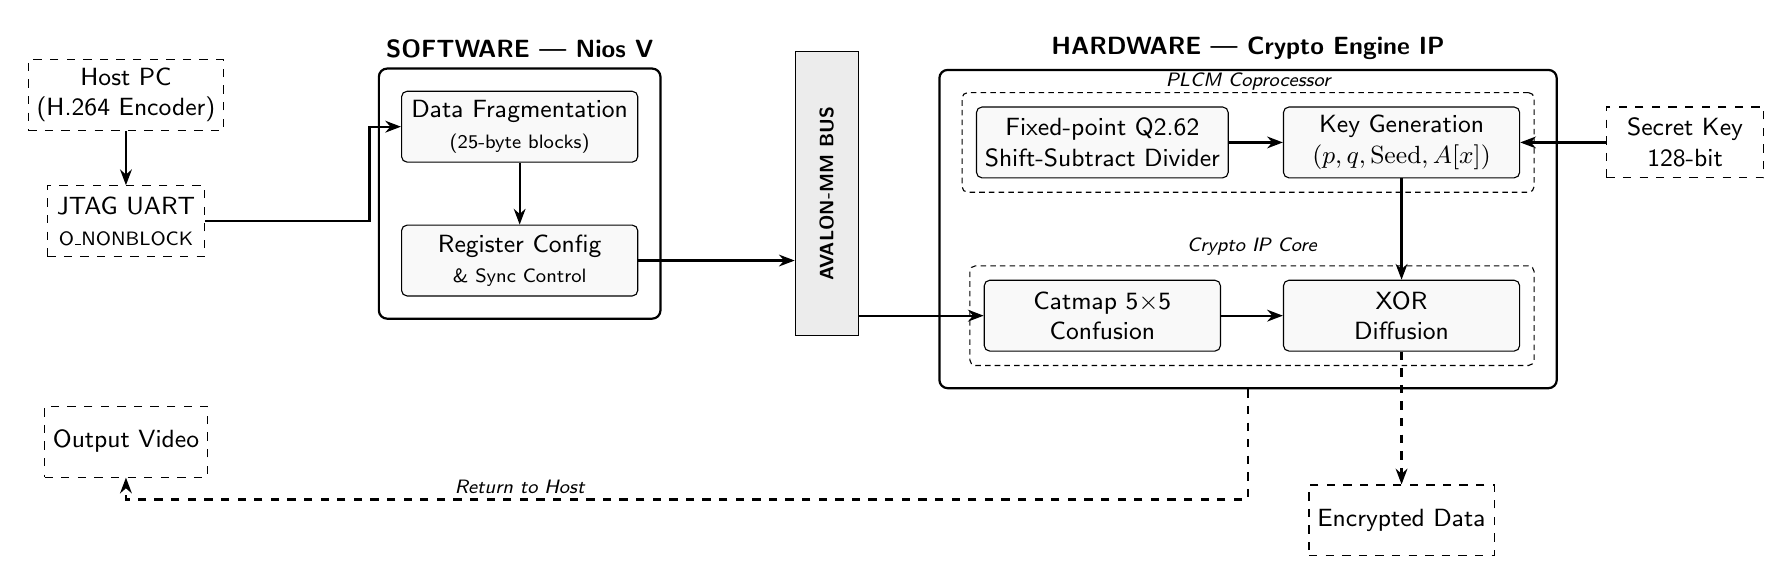
\begin{tikzpicture}[
    font=\sffamily\small,
    >={Stealth[length=2mm]},
    block/.style={draw, rectangle, rounded corners=2pt, align=center,
                  minimum height=9mm, minimum width=30mm, inner sep=3pt,
                  fill=gray!5},
    ext/.style={draw, rectangle, dashed, align=center,
                minimum height=9mm, minimum width=20mm, inner sep=3pt},
    group/.style={draw, thick, rounded corners=3pt, inner sep=8pt},
    subgroup/.style={draw, thin, rounded corners=2pt, inner sep=5pt,
                     dash pattern=on 2pt off 1.5pt},
    arr/.style={->, thick},
    darr/.style={->, thick, dashed},
    lab/.style={font=\sffamily\scriptsize\itshape, inner sep=1pt},
]

% ===== Software blocks =====
\node[block] (frag) at (0,0)    {Data Fragmentation\\\scriptsize(25-byte blocks)};
\node[block] (reg)  at (0,-1.7) {Register Config\\\scriptsize \& Sync Control};
\node[group, fit=(frag)(reg),
      label={[font=\sffamily\bfseries\small]above:SOFTWARE --- Nios V}] (sw) {};

% ===== Host side (left) =====
\node[ext] (host) at (-5, 0.4)  {Host PC\\(H.264 Encoder)};
\node[ext] (jtag) at (-5,-1.2)  {JTAG UART\\\scriptsize O\_NONBLOCK};
\node[ext] (outv) at (-5,-4.0)  {Output Video};

% ===== Bus =====
\node[draw, fill=gray!15, minimum width=8mm, minimum height=36mm,
      align=center] (bus) at (3.9,-0.85) {};
\node[rotate=90, font=\sffamily\bfseries\scriptsize] at (bus.center) {AVALON-MM BUS};

% ===== Hardware: PLCM Coprocessor (lowered) =====
\node[block] (div) at (7.4, -0.2)   {Fixed-point Q2.62\\Shift-Subtract Divider};
\node[block] (key) at (11.2, -0.2)  {Key Generation\\$(p,q,\mathrm{Seed},A[x])$};
\node[subgroup, fit=(div)(key),
      label={[font=\sffamily\itshape\scriptsize, yshift=-1mm]above:PLCM Coprocessor}] (plcm) {};

% ===== Hardware: Crypto IP Core =====
\node[block] (cat) at (7.4, -2.4)  {Catmap 5$\times$5\\Confusion};
\node[block] (xor) at (11.2,-2.4)  {XOR\\Diffusion};
\node[subgroup, fit=(cat)(xor),
      label={[font=\sffamily\itshape\scriptsize]above:Crypto IP Core}] (crypto) {};

% ===== Hardware outer group =====
\node[group, fit=(plcm)(crypto),
      label={[font=\sffamily\bfseries\small]above:HARDWARE --- Crypto Engine IP}] (hw) {};

% ===== Right / bottom externals =====
\node[ext] (skey) at (14.8, -0.2) {Secret Key\\128-bit};
\node[ext] (enc)  at (11.2,-5.0)  {Encrypted Data};

% ===== Host -> Software via JTAG =====
\draw[arr] (host) -- (jtag);
\draw[arr] (jtag.east) -| ($(frag.west)+(-0.4,0)$) -- (frag.west);

% ===== Software flow =====
\draw[arr] (frag) -- (reg);

% ===== Software -> Bus -> Crypto IP Core only =====
\draw[arr] (reg.east) -- (reg.east -| bus.west);
\draw[arr] (bus.east |- cat.west) -- (cat.west);

% ===== PLCM internal =====
\draw[arr] (div) -- (key);
\draw[arr] (skey) -- (key);

% ===== Keystream feeds Crypto =====
\draw[arr] (key.south) -- (xor.north);

% ===== Crypto internal =====
\draw[arr] (cat) -- (xor);

% ===== Encrypted Data out =====
\draw[darr] (xor.south) -- (enc.north);

% ===== Return path: HW -> bottom -> Output Video =====
\draw[darr] (hw.south) -- ++(0,-1.4) -| (outv.south)
            node[pos=0.55, above, lab, xshift=50mm] {Return to Host};

\end{tikzpicture}
\end{document}